% xetex compatible variant that support TTF fonts according to company rules
\documentclass[ignorenonframetext, professionalfonts, hyperref={unicode}]{beamer}

\usetheme{Epam}

\usepackage{fontspec}
\setsansfont{SourceSansPro-Regular}
%\setbeamerfont{frametitle}{family=\fontspec{Oswald}}
\setbeamerfont{frametitle}{family=\fontspec{Oswald}}
\setbeamerfont{block title}{family=\fontspec{Oswald}}

%\setmainfont{Times New Roman}
\defaultfontfeatures{Mapping=tex-text}
\defaultfontfeatures{Ligatures=TeX}

%\setsansfont{Arial}
%\setromanfont{Trebuchet MS}

\usepackage{cmap}
\usepackage{graphicx}

\usepackage{textcomp}

\usepackage{beamerthemesplit}

\usepackage{ulem}

\usepackage{verbatim}
\usepackage{import}

\usepackage{listings}
\lstloadlanguages{bash}

\lstset{escapechar=`,
	captionpos=b,
	extendedchars=false,
	language=sh,
%	frame=single,
	tabsize=2, 
	columns=fullflexible, 
%	basicstyle=\scriptsize,
	keywordstyle=\color{blue}, 
	commentstyle=\itshape\color{brown},
%	identifierstyle=\ttfamily, 
	stringstyle=\mdseries\color{green}, 
	showstringspaces=false, 
	numbers=left, 
	numberstyle=\footnotesize, 
	breaklines=true, 
	inputencoding=utf8,
	keepspaces=true,
	morekeywords={u\_short, u\_char, u\_long, in\_addr}
	}

\definecolor{darkgreen}{cmyk}{0.7, 0, 1, 0.5}

\lstdefinelanguage{diff}
{
    morekeywords={+, -},
    sensitive=false,
    morecomment=[l]{//},
    morecomment=[s]{/*}{*/},
    morecomment=[l][\color{darkgreen}]{+},
    morecomment=[l][\color{red}]{-},
    morestring=[b]",
}

\author[Epam]{{\bf Epam}\\Low Level Programming Department}

%\institution[EPAM]{EPAM}
%\logo{\includegraphics[width=1cm]{logo.png}}

\graphicspath{{../../slides/cmdline/clipart/}{../../slides/bash/clipart/}}

\bibliographystyle{unsrt}
\setbeamertemplate{bibliography item}{\insertbiblabel}

\AtBeginSection[]{%
  \begin{frame}<beamer>
    \frametitle{}
    \tableofcontents[
        sectionstyle=show/shaded, hideallsubsections ]
  \end{frame}
  \addtocounter{framenumber}{-1}% If you don't want them to affect the slide number
}

% \regex for regular expressions
\newcommand{\regex}[1]{ %
\expandafter{$\ulcorner{\color{blue}\texttt{#1}}\lrcorner$} %
}



\title{Введение в GNU/Linux}

%%%%%%%%%%%%%%%%%%%%%%%%%%%%%%%%%%%%%%%%%%%%%%%%%
%%%%%%%%%% Begin Document  %%%%%%%%%%%%%%%%%%%%%%
%%%%%%%%%%%%%%%%%%%%%%%%%%%%%%%%%%%%%%%%%%%%%%%%%

\begin{document}

\begin{frame}
	\frametitle{Network file systems}
	\titlepage
	\vspace{-0.5cm}
	\begin{center}
	%\frontpagelogo
	\end{center}
\end{frame}


\begin{frame}
	\tableofcontents
	[hideallsubsections]
\end{frame}

%%%%%%%%%%%%%%%%%%%%%%%%%%%%%%%%%%%%%%%%%   
%%%%%%%%%% Content starts here %%%%%%%%%%
%%%%%%%%%%%%%%%%%%%%%%%%%%%%%%%%%%%%%%%%%

\section{NFS}
\mode<all>{\begin{frame}
    \frametitle{Network Attached Storage vs Storage Attached Network}
    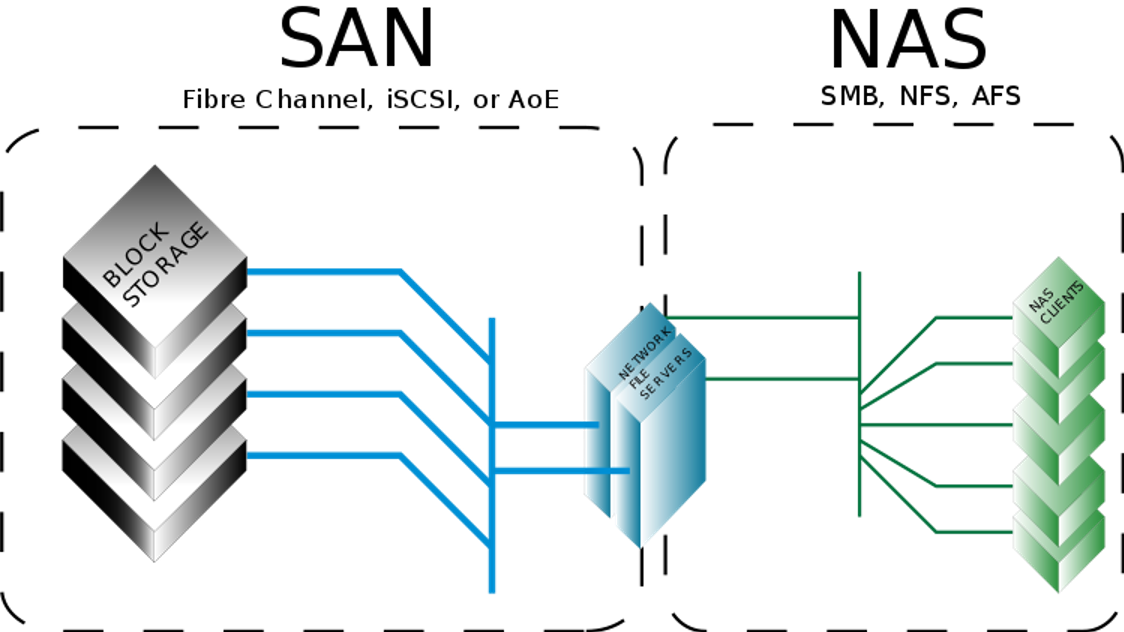
\includegraphics[height=6cm]{../../slides/nfs/images/sannas.png}

\end{frame}}
\mode<all>{\begin{frame}
    \frametitle{Network File System (NFS)}
    Позволяет подключать (монтировать) удалённые файловые системы через сеть.
\begin{itemize}
    \item Клиент/сервер
    \item UDP/TCP
    \item версии v3, v4, v4.1 
    \item встроена в ядро Linux
    \item поддержка на Unix-подобных системах (BSD / Linux / Android / OS X)
\end{itemize}
    

\end{frame}}
\mode<all>{\begin{frame}
    \frametitle{Применение NFS}

    \begin{itemize}
        \item Домашняя директория /home/ на несколько компьютеров
        \item Доступ для загрузки ISO образа на удаленном сервере IPMI (iDRAC).
        \item Обновление firmware с сетевого хранилища
        \item Бездисковые хосты/бездисковая загрузка (NFS - на корневом разделе)
        \item k8s может использовать в качестве volume NFS 
        \item при балансировке нагрузки общее хранилище корневой директории
    \end{itemize}

\end{frame}}
\mode<all>{\begin{frame}
    \frametitle{Недостатки}
    \begin{itemize}
        \item безопасность (трафик не шифруется), но есть возможность настроить Kerberos
        \item синхронизация пользователей между хостами
        \item из за RPC (Remote Procedure Call) - много открытых портов на firewall
    \end{itemize}

\end{frame}}
\mode<all>{\begin{frame}[fragile]
    \frametitle{Доступ к сети}

Синтаксис /etc/exports:

\begin{lstlisting}
<full_path>  <network> (<options>)
\end{lstlisting}

Примеры поля <network>:
    \begin{itemize}
        \item 192.168.0.0/255.255.255.0
        \item 192.168.0.0/24
        \item 192.168.0.29
        \item 192.168.0.*
        \item 192.168.0.10?
        \item *
        \item *.domain.com
    \end{itemize}
    

\end{frame}}
\mode<all>{\begin{frame}[fragile]
    \frametitle{Настройки}
   options
    \begin{itemize}
        \item ro 
        \item rw
        \item async
        \item sync
        \item roout\_squash
        \item no\_root\_squash
    \end{itemize}

\end{frame}}
\mode<all>{\begin{frame}
    \frametitle{Команды диагностики}
\begin{itemize}
    \item 
    exportfs -a Экспортировать все каталоги
    \item 
    exportfs -v Показывать процесс экспорта
    \item 
    exportfs -u Отменить экспорт одного и более каталогов
    \item showmount -a or mount 
    Вывести список всех удаленных монтирований в формате: hostname:directory, где hostname - имя клиента, а directory - корень монтированной файловой системы
    \item 
    showmount -d Вывести список каталогов, смонтированных клиентами на удалении
    \item 
    showmount -e Вывести список экспортированных файловых систем
    \item 
    nfsstat
    Статистика работы nfs сервера
\end{itemize}
     

\end{frame}}
\mode<all>{\begin{frame}[fragile]
    \frametitle{Пример автомонтирования}
\begin{lstlisting}
cat /etc/fstab
10.0.0.10:/var/nfs_share /mnt/nfs_share  nfs \
_netdev,noauto,x-systemd.automount,x-systemd.mount-timeout=10,timeo=14,x-systemd.idle-timeout=1min 0 0
\end{lstlisting}

\begin{lstlisting}
systemctl daemon-reload
systemctl restart remote-fs.target
ls /mnt/nfs_share/
findmnt -t nfs4
\end{lstlisting}

\end{frame}}
\section{CIFS}
\mode<all>{\begin{frame}
    \frametitle{Server Message Block/Common Internet File System}
    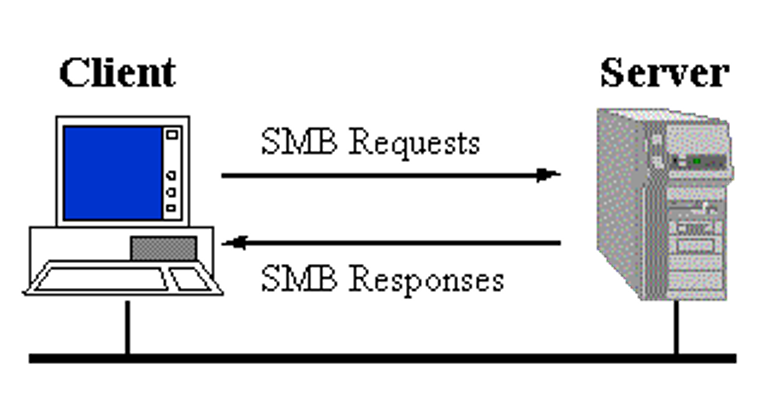
\includegraphics[height=6cm]{../../slides/smb/images/smb.png}
\end{frame}}
\mode<all>{\begin{frame}
    \frametitle{Server Message Block (SMB) }
 Server makes available to clients on the network
  \begin{itemize}
      \item files 
      \item printers 
      \item serial ports
      \item API
  \end{itemize}  

Connection: NetBIOS over TCP/IP

Send commands: Server Message Block (SMB)


\end{frame}}
\mode<all>{\begin{frame}
    \frametitle{Пакет Samba}

    Интеграция Linux/Unix серверов в Active Directory
    \begin{itemize}
        \item 
    \end{itemize}

    Клиенты: smbclient, smbfs
    
    Сервер предoставляет:
    \begin{itemize}
        \item NetBIOS over TCP/IP (NBT)
        \item SMB (known as CIFS in some versions)
        \item A WINS server also known as a NetBIOS Name Server (NBNS)
        \item The NT Domain suite of protocols which includes NT Domain Logons
        \item Active Directory Logon using modified versions of Kerberos and LDAP.
    \end{itemize}
    

\end{frame}}
\section{IPFS}

\end{document}
